\documentclass{article}
\usepackage[utf8]{inputenc}
\usepackage{geometry}
\usepackage{graphicx}
\usepackage{pgfplots}
\usepackage{amsmath}
\usepackage{amssymb}
\usepackage{amsfonts}
\usepackage{mdframed}
\usepackage{amsthm}
\usepackage{physics}
\usepackage{derivative}
\usepackage{hyperref}
\renewcommand{\theenumi}{\roman{enumi}}

\geometry{a4paper, left=2cm, right=2cm, top=1cm, bottom=2cm}

\pgfplotsset{compat=1.18}
\begin{document}

\begin{minipage}{0.7\textwidth}
    \small \textbf{LABORATORIO DE MECÁNICA VECTORIAL}  \\
    \small {Facultad de Ciencias, Universidad Nacional Autónoma de México} \\
    \small {Profesor: Radamés Ricardo Reynoso Manríquez} \\
    \small {Ayudante: Ana Laura Córdova Lara}\\
    \small {Fecha de entrega: 17 de Abril de 2024} \\
    \small {Nombre completo: Andrés López González} \\
    \small {Tarea número VIII}
\end{minipage}
\hfill
\begin{minipage}{0.12\textwidth}
    
\includegraphics[width=\linewidth]{logo_universidad}
\end{minipage}

\section*{Cuestionario VIII}
Pregunta 1. Un abanico que está girando, completa 1200 revoluciones cada minuto. Considere un punto en la punta de un aspa, la cual tiene un radio de 0.15 m. (a) ¿A qué distancia se mueve el punto en una revolución? \textbf{Dado que hablamos de una trayectoria circular entonces para obtener la distancia recorrida en una revolución es el perímetro del círculo, que se determina como $\pi d = 2\pi 0.15m \approx 0.94247m$} (b) ¿Cuál es la velocidad del punto? \textbf{Al no especificar en qué unidades pide la velocidad usaremos RPM que es la que da cantidades más exactas, siendo la velocidad 1,200 RPM, en metros sobre minuto es simplemente el perímetro que recorre en una revolución multiplicado por 1,200 y dividido en 60 segundos quien es aproximadamente $18.84955 \frac{m}{s}$} (c) ¿Cuál es su aceleración? \textbf{La aceleración angular no existe pues en cada giro recorre las mismas revoluciones en tiempos iguales, por tanto la aceleración tangencial tampoco existe, la aceleración centrípeta en cambio sí existe pues es la que mantiene la atracción al centro siendo esta $a_c = \frac{v^2}{r} \approx \frac{18.84955^2\frac{m^2}{s^2}}{0.15s} \approx 2,368.70356\frac{m}{s^2} $}\\\\

Pregunta 2. Se cree que ciertas estrellas de neutrones (estrellas extremadamente densas)
giran alrededor de 1 rev/seg. Si una estrella tal tiene un radio de 20 km (valor típico), (a) ¿cuál es la velocidad de un punto situado en el ecuador de la estrella? \textbf{Anteriormente resolvimos algo muy similar, una revolución es $\pi d = 2 \pi 20km = 40 \pi km$, ahora como son revoluciones sobre segundos es simplemente dividir esto sobre un segundo por lo que su velocidad es $40 \pi \frac{km}{s} \approx 125.6637 \frac{km}{s}$} (b) ¿cuál es la aceleración centrípeta de ese punto? \textbf{Sabiendo esta velocidad solo sustituimos en la fórmula anterior $a_c = \frac{v^2}{r} = \frac{\left(40\:\pi \right)\:^2}{20} \frac{km}{s^2} = 80 \pi^2 \frac{km}{s^2} \approx 789.5683 \frac{km}{s^2}$}\\\\
Pregunta 3. Explique en detalle la diferencia entre la naturaleza de la aceleración tangencial, aceleración centrípeta, y aceleración centrífuga.\\
\textbf{I.} \textit{Aceleración Tangencial}: Esta aceleración se refiere a los cambios en la magnitud de la velocidad de un objeto en movimiento circular. Imagina un objeto que se mueve en un círculo a velocidad constante. Aunque su velocidad no cambia, su dirección sí lo hace constantemente, por lo que experimenta una aceleración. La aceleración tangencial es la componente de la aceleración total que está en la dirección de la tangente al círculo en cualquier punto dado. Matemáticamente, la aceleración tangencial se puede expresar como la derivada temporal de la magnitud de la velocidad, es decir, $a_t = \frac{dv}{dt}$, donde $v$ es la velocidad y $t$ es el tiempo.

\noindent \textbf{II.} \textit{Aceleración Centrípeta}: Esta aceleración se refiere a los cambios en la dirección de la velocidad de un objeto en movimiento circular. En un movimiento circular uniforme, la velocidad del objeto cambia continuamente de dirección, lo que significa que está experimentando una aceleración hacia el centro del círculo. Esta aceleración es responsable de mantener al objeto en su trayectoria circular. La aceleración centrípeta siempre apunta hacia el centro del círculo con la misma dirección del vector área y su magnitud se puede calcular utilizando la fórmula $a_c = \frac{v^2}{r}$, donde $v$ es la velocidad tangencial y $r$ es el radio de la trayectoria circular; es la causante de que los vectores unitarios base de la función posición vectorial cambien a lo largo del tiempo.

\noindent \textbf{III.} \textit{Aceleración Centrífuga}: A menudo, se habla de la "fuerza centrífuga", que es una fuerza ficticia que parece empujar un objeto hacia afuera desde el centro de rotación en un sistema de referencia no inercial. Sin embargo, en el contexto de la aceleración, la aceleración centrífuga no es una aceleración real. Es simplemente la sensación de "fuerza" que experimenta un objeto en movimiento circular desde su propio marco de referencia. En otras palabras, cuando estás dentro de un vehículo que gira en una curva, sientes que estás siendo "empujado" hacia afuera, pero en realidad, tu cuerpo está tratando de continuar moviéndose en línea recta debido a la inercia. La aceleración centrífuga no es más que la fuerza de inercia percibida desde el sistema de referencia en rotación.\\\\

Pregunta 4. (a) ¿Cuál es la aceleración centrípeta de un objeto situado en el ecuador de la Tierra debido a la rotación de la misma? \textbf{La velocidad tangencial en el ecuador es $464.82 \frac{m}{s}$ y el radio a este es $6,378km$, $a_c = \frac{v^2}{r^2} = \frac{\left(464.82 \frac{m}{s}\right)^2}{6.378 \cdot 10^6 m} \approx 0.03387 \frac{m}{s^2}$} (b) ¿Cuál tendría que ser el período de rotación de la Tierra para que los objetos situados en el ecuador tuvieran una aceleración centrípeta igual a 9.8 m/s2? \textbf{Recordemos que el radio de la tierra es aproximadamente de 6,378km, se ve que el camino por el que va esta pregunta es relacionar con la aceleración de atracción gravitacional así que fijamos $a_c = 9.8066\frac{m}{s} = g$. Como $a_c = \dfrac{v^2}{r} = \dfrac{\left(\dfrac{2\pi r}{T}\right)^2}{r} = \dfrac{(2\pi r)^2}{T^2r}$ entonces tenemos que $T = \sqrt{\dfrac{(2\pi r)^2}{a_cr}} = \dfrac{2\pi \sqrt{r}}{\sqrt{a_c}} = \dfrac{2\pi\sqrt{6.378 \cdot 10^6 m}}{\sqrt{9.8066\frac{m}{s^2}}} \approx 8,067.13990s \approx 22.40872hrs $}  \\\\
Pregunta 5. Una partícula está viajando en una trayectoria circular de 3.64 m de radio. En cierto instante, la partícula se mueve a razón de 17.4 m/s, y su aceleración forma un ángulo de 22° en dirección al centro del círculo según se ve desde la partícula (figura 1).\\
\begin{figure}[h]
    \centering
    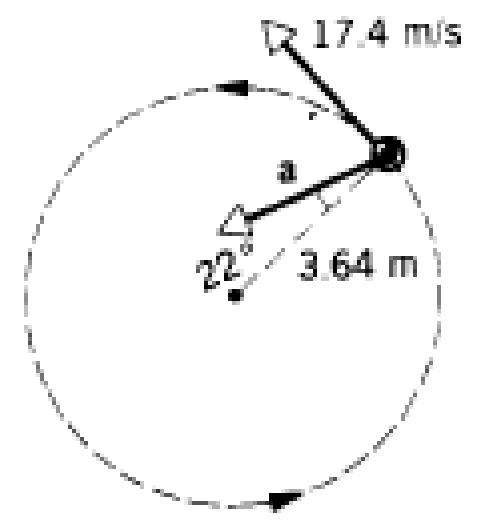
\includegraphics[width=0.25\linewidth]{Circle.png}
    \caption{Descripción del movimiento.}
    \label{fig:enter-label}
\end{figure}\\
¿A qué tasa está creciendo la velocidad de la partícula? ¿Cuál es la magnitud de la aceleración? \textbf{Debemos calcular la aceleración que siente este movimiento derivada de $a_c = a \sin(90-\vartheta) = a\sin(68)$ de modo que $a = \frac{a_c}{\sin(68)} = \frac{\frac{v^2}{r}}{\sin(68)} = \frac{v^2}{r \sin(68)} = \frac{(17.4ms^{-1})^2}{\sin(68) \cdot 3.64m} \approx 89.70801 \frac{m}{s^2}$, esto fue la magnitud pero la aceleración centrípeta ya ha sido calculada en el proceso, explicitaremos este paso pero de forma más rápida conociendo $|a_c|=a$ $a_c = a \sin(68) \approx 83.17582 \frac{m}{s^2}$}.\\\\

\noindent Pregunta 6. Una partícula se mueve en un plano de acuerdo a
$$x = R \sin \omega t + \omega Rt$$
$$y = R cos \omega t + R$$
donde ω y R son constantes. Esta curva, llamada cicloide, es la trayectoria trazada por
un punto de la llanta de una rueda que gira sin resbalamiento a lo largo del eje x. (a) Trace la trayectoria.\\
\begin{figure}[h]
    \centering
    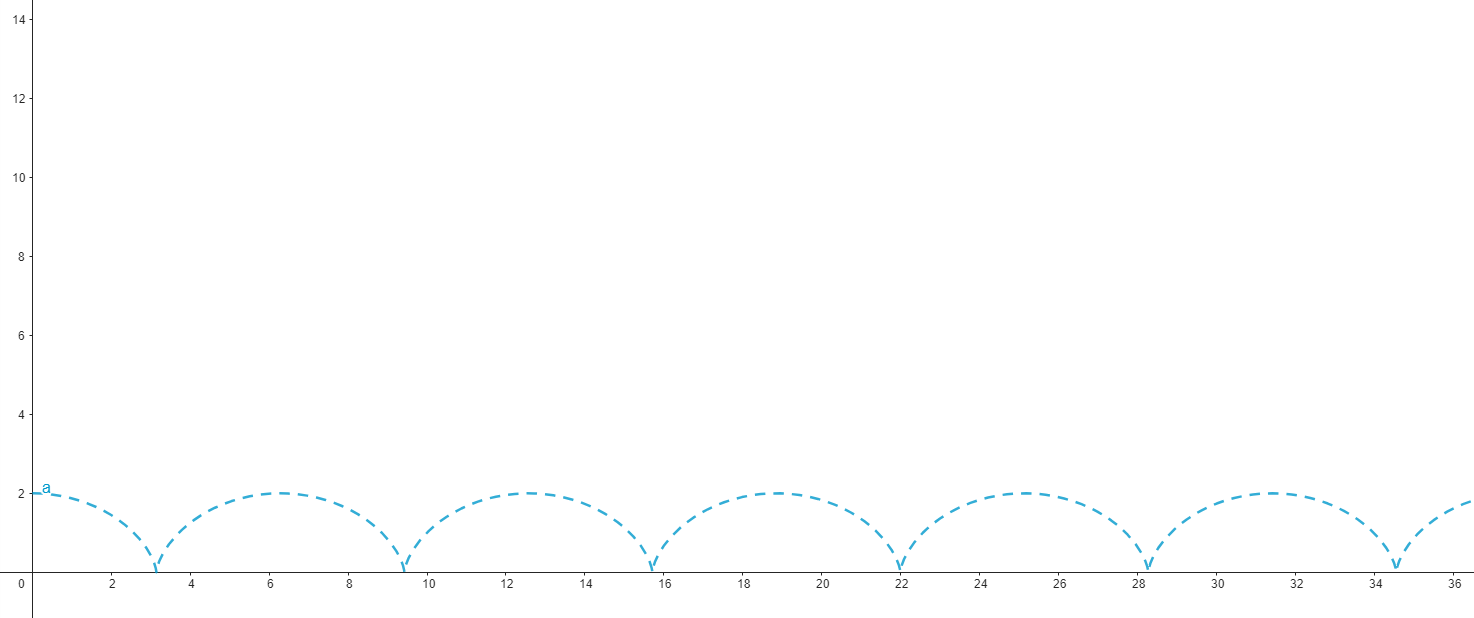
\includegraphics[width=0.5\linewidth]{Cicloide.png}
    \caption{Cicloide: R=1}
    \label{fig:enter-label}
\end{figure}\\
(b) Calcule la velocidad y la aceleración instantáneas cuando la partícula está en el valor de y máximo y mínimo. \\
\textbf{Considérese la parametrización dada de parejas ordenadas $(x,y) = (R \sin \omega t + \omega Rt, R \cos \omega t + R)$, consideremos la restricción del tiempo y la oscilación de omega tal que $\omega,t \in [0,2\pi)$, notemos que es continua y simétricamente suryectiva además de que al estar restringida existe un máximo y mínimo que por su naturaleza los máximos indican los puntos de velocidad cero y los mínimos de tasa de cambio en su velocidad extremadamente rápida, diferenciamos en este intervalo de modo que obtenemos $(x',y') = (\omega tR \cos(\omega t)+\omega R, R\omega t \sin(\omega t)) = \Vec{0}$}, por lo aprendido el Geometría Analítica I igualamos entrada a entrada y obtenemos las siguientes raíces generalizadas: $2\mathbb{Z}R\pi, (2+1)\mathbb{Z}R\pi$. Por la gráfica que hemos trazado es evidente que $2\mathbb{Z}R\pi$ corresponde a los máximos (velocidad cero) y $(2+1)\mathbb{Z}R\pi$ a los mínimos (velocidad que tiende a $\pm \infty$), con esta generalización y solo usando la derivada paramétrica (aunque la derivada material hubiera sido igual de buena) obtenemos todos los máximos y mínimos para $\omega,t \in \mathbb{R}$ de modo que (trivialmente pero remarcable) $2\mathbb{Z}$ se refiere a los números pares mientras que $(2+1)\mathbb{Z}$ a los impares. La derivada paramétrica de segundo orden nos puede dar la aceleración pero por nuestros cursos de Cálculo es evidente que al oscilar entre senos y cosenos solo cambiará en $2\mathbb{Z}R\pi$ (es interesante que solo intercambian posiciones entre seno y coseno pues por cuestiones de imparidad/paridad del seno/coseno con un poco de álgebra quedan las mismas funciones) por lo cual la aceleración máxima es en $(2+1)\mathbb{Z}R\pi$ mientras que la mínima en $2\mathbb{Z}R\pi$.
\begin{figure}
    \centering
    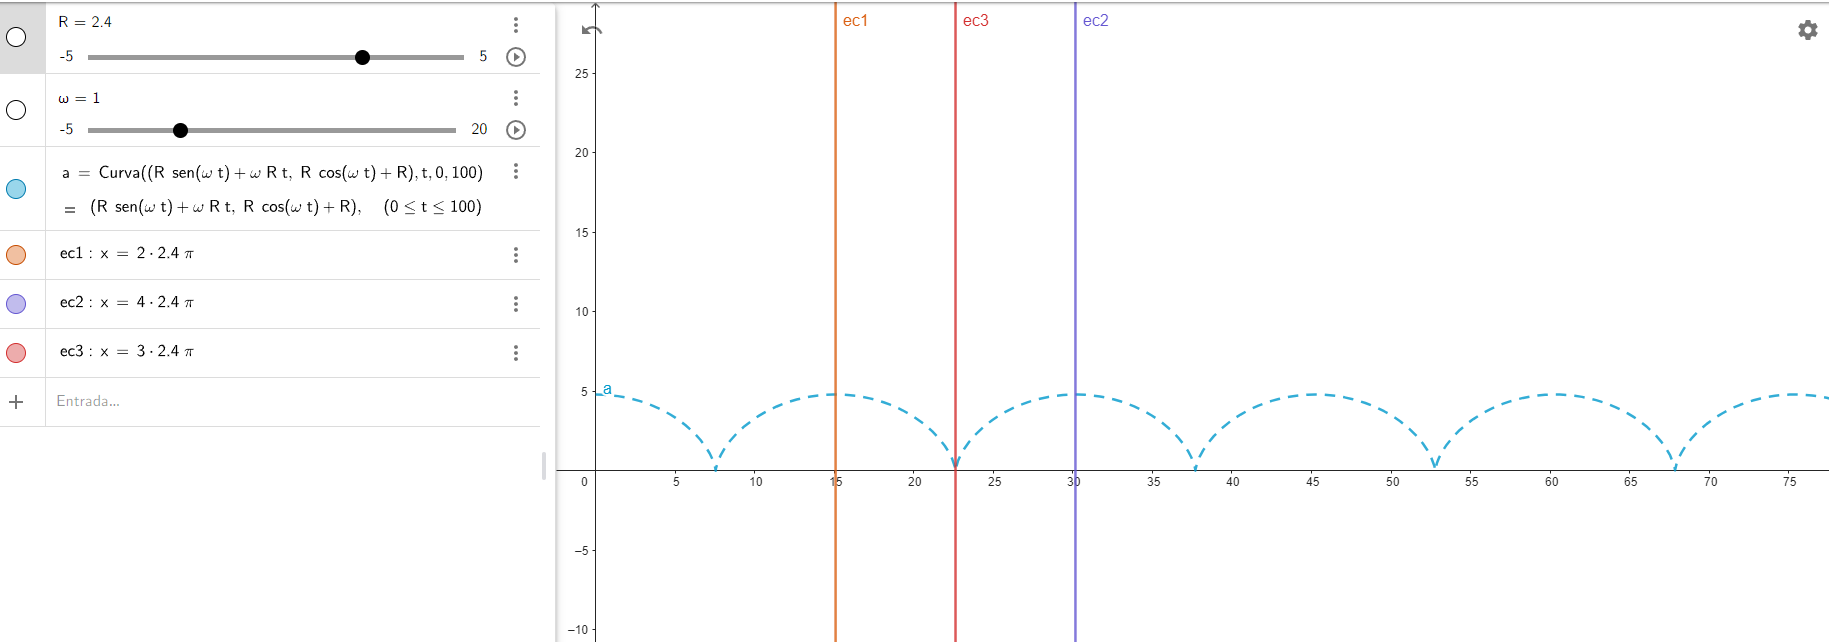
\includegraphics[width=0.5\linewidth]{demo.png}
    \caption{Demostración que funciona para todo valor de omega, R, tiempo.}
    \label{fig:enter-label}
\end{figure}



\end{document}
